\documentclass[tikz]{standalone}

\usepackage{bbold}		    % Za identiteto
\usepackage{amsmath}		    % Matematicni izrazi
\usepackage{pgf}		    % I guess da za risat slike
\usepackage{tikz}		    % Tikz
\usepackage[english,slovene]{babel} % Jezik
\usepackage[utf8]{inputenc}	    % Encoding

\usetikzlibrary{arrows,automata}    %
\usetikzlibrary{positioning}

\let\oldhat\hat
\renewcommand{\vec}[1]{\mathbf{#1}}
\renewcommand{\hat}[1]{\oldhat{\mathbf{#1}}}


\tikzset{ 
    state/.style={ 
	rectangle, 
	sharp corners, 
	draw=black, thick, 
	minimum height=1em, 
	inner sep=2pt, 
	align = center, 
	},
    line/.style ={ 
	draw, 
	thick, 
	-latex',
	}.
    }
%\tikzstyle{line} = [draw, -latex']

\begin{document}

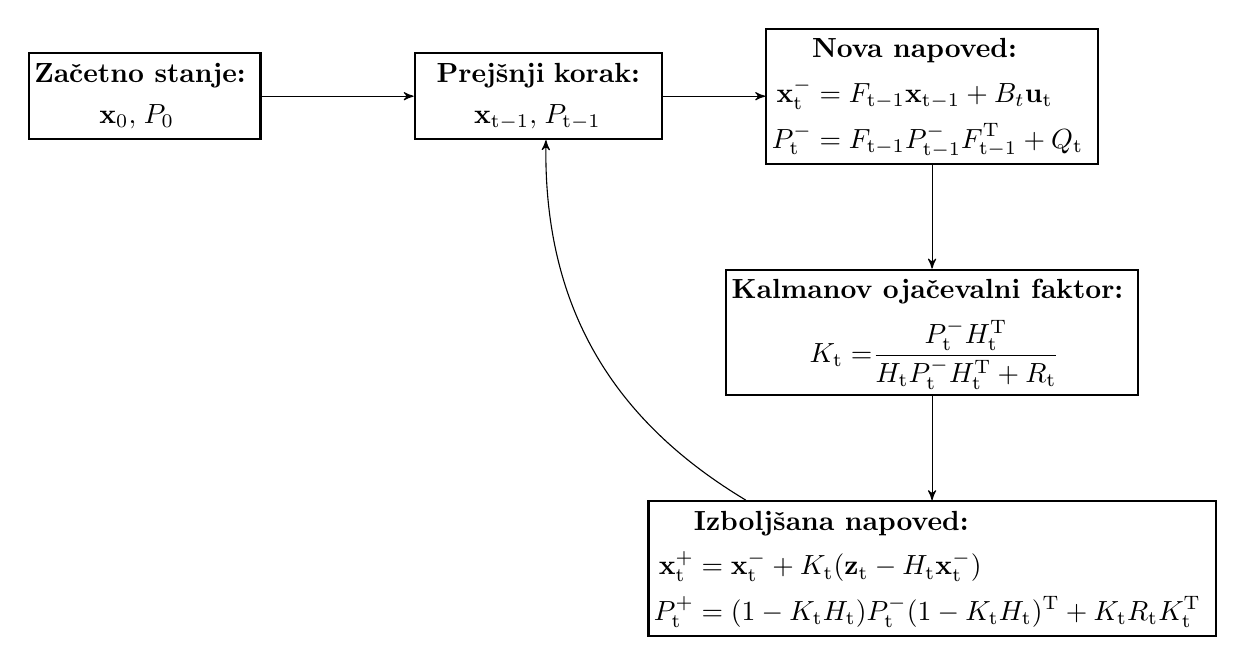
\begin{tikzpicture}[->,>=stealth']

% Zacetno stanje
\node[state, rectangle] (ena) 
    {$\begin{aligned} 
	\textbf{Začetno} & \textbf{ stanje:}\\ 
	\vec{x}_0, \; &P_0 
    \end{aligned}$ 
    };
  
% Prejsnji korak
\node[state,    	% layout (defined above)
    rectangle,		% rectangle 
    text width=3cm, 	% max text width 
    %yshift=2cm, 		% move 2cm in y 
    right of=ena, 	% Position is to the right of QUERY 
    node distance=5cm, 	% distance to QUERY 
    anchor=center] (dva) 	% posistion relative to the center of the 'box'
    {%
	$\begin{aligned} 
	    \textbf{Prejšnji} &\textbf{ korak:}\\ 
	    \vec{x}_{\text{t}-1}, \; &P_{\text{t}-1} 
	\end{aligned}$ 
    };
 
% Nova napoved
\node[state, 
    rectangle, 
    right of=dva, 
    node distance=5cm, 
    anchor=center] (tri) 
    {% 
	$\begin{aligned} 
	    &\textbf{Nova napoved:}\\ 
	    \vec{x}_{\text{t}}^- &= F_{\text{t}-1}\vec{x}_{\text{t}-1} + B_t 
				    \vec{u}_{\text{t}}\\ 
	    P_{\text{t}}^- &= F_{\text{t}-1} P_{\text{t}-1}^- F_{\text{t}-1}^{\text{T}} + 
				Q_{\text{t}} 
	\end{aligned}$ 
    };
% Kalmanov faktor
\node[state, 
    rectangle, 
    below of=tri, 
    yshift=-2cm, 
    anchor=center] (stiri) 
    {% 
	$\begin{aligned} 
	    \textbf{Kalmanov} &\textbf{ ojačevalni faktor:}\\ 
	    K_{\text{t}} = &\frac{ P_{\text{t}}^- H_{\text{t}}^{\text{T}}}{H_{\text{t}} 
			    P_{\text{t}}^- H_{\text{t}}^{\text{T}} + R_{\text{t}}} 
	\end{aligned}$ 
    };

% Izobljšana napoved
\node[state, 
    rectangle, 
    below of=stiri, 
    yshift=-2cm, 
    anchor=center] (pet) 
    {% 
	$\begin{aligned} 
	    &\textbf{Izboljšana} \textbf{ napoved:}\\ 
	    \vec{x}_{\text{t}}^+ &= \vec{x}_{\text{t}}^- + K_{\text{t}} (\vec{z}_{\text{t}} 
				    - H_{\text{t}} \vec{x}_{\text{t}}^-) \\ 
	    P_{\text{t}}^+ &= (\mathbb{1} - K_{\text{t}}  H_{\text{t}}) P_{\text{t}}^-
				(\mathbb{1} - K_{\text{t}}  H_{\text{t}})^{\text{T}} +
				K_{\text{t}} R_{\text{t}} K_{\text{t}}^{\text{T}} 
	\end{aligned}$ 
    }; 

\path[]
    (ena) edge node [right] {} (dva)
    (dva) edge node [right] {} (tri)
    (tri) edge node {} (stiri)
    (stiri) edge node {} (pet)
    (pet) edge [bend left] node[left] {} (dva);
                             
\end{tikzpicture}
\end{document}
